\section{Трекинг на основе особых точек и цвета}\label{tracking}

Данный раздел содержит описание предлагаемого алгоритма трекинга,
комбинирующего в себе два подхода: основанный на ключевых точках
и основанный на цветах.
Сначала идет описание части метода, использующей точечные особенности
изображения.
Оно достаточно кратко, поскольку рассказывает о довольно
распространенном и известном подходе.
Затем идет описание части, использующей цветовую информацию.
Оно более подробно, поскольку касается менее распространённого подхода и
содержит некоторые модификации.
Завершается раздел описанием способа комбинирования цветового и точечного
алгоритмов.

\subsection{Трекинг на основе точечных особенностей изображения}
\label{subs:feat_tracking}

Применяемый в данной работе алгоритм трекинга с помощью точечных особенностей
представляет собой разновидность стандартного подхода "--- трекера
Канаде "--- Лукаса "--- Томаси
(KLT-трекера)\cite{LucasAndKanade,TomasiAndKanade,ShiAndTomasi,PyrLK}.
На кадрах с известной позицией объекта выделяются ключевые 2D-точки (точечные
особенности) и определяются соответствующие им 3D-точки на поверхности модели.
Движение ключевых точек от кадра к кадру отслеживается с помощью вычисления
оптического потока.

На кадре, для которого выполняется оценка позиции, по известным 2D-3D
соответствиям вычисляется положение объекта путем решения задачи
\PnP\cite{LepetitSurvey} с использованием RANSAC\cite{RANSAC} для отсеивания
выбросов.
После определения позиции объекта на очередном кадре производится
регистрация ключевых точек на областях изображения, не покрытых
уже известными точками.
Таким образом, каждая особенность отслеживается на протяжении
нескольких кадров, пока это возможно.
Набор 2D-координат одной и той же ключевой точки в совокупности с ее
3D-координатами называется \term{треком}.

Дополнительные подробности работы с точечными особенностями описаны далее,
в разделе~\ref{combining}.

\subsection{Метод на основе распределения цвета}

\Comment{Во всем разделе надо провести ревизию обозначений и формул.}

Использующий распределение цветов метод направлен на нахождение такой
позиции, при которой контур наилучшим образом отделяет передний план от фона.
Это означает, что цвета на $\FgProj$ будут соответствовать цветам,
ранее встречавшимся на переднем плане в ходе трекинга, и наоборот:
оказавшиеся на $\BgProj$ точки будут иметь цвет, характерный для фона.

После вычисления позиции объекта на каждом кадре собираются данные о цветах
точек на переднем плане и на фоне.
Затем эти данные объединяются с собранной в ходе трекинга общей статистикой.
Статистика собирается в окрестности контура объекта.
Эта окрестность, обозначаемая $\CtLocal$, разбивается на $\CtLocalCnt$
непересекающихся областей~$\CtLocal_1, \dots, \CtLocal_\CtLocalCnt$.
Каждая из этих областей включает в себя часть переднего плана и часть фона:
\begin{align}\label{eqn:histo_partitioning}
    \CtLocalI &= {\CtLocalFgI} \sqcup {\CtLocalBgI} \\
    {\CtLocalFgI} &= \CtLocalI \cap \CtLocalFg \\
    {\CtLocalBgI} &= \CtLocalI \cap \CtLocalBg
\text{.}
\end{align}
О разбиении окрестности контура на локальные области подробнее рассказано в
разделе \ref{local-areas}.

Цветовая статистика ведётся для каждой из областей ${\CtLocalFgI}$ и
${\CtLocalBgI}$ отдельно, для того чтобы отдельно учитывать цветовые
особенности разных сторон объекта.
Для её хранения и обновления используются гистограммы распределения цветов.
Перед построением гистограмм изображение преобразуется так, чтобы цвет в каждом
канале принимал целочисленные значения от $0$ до $31$.
Таким образом, каждая гистограмма состоит из $32^3$ ячеек.
В каждую ячейку гистограмм ${\HistLocalFg}$ и $\HistLocalBg{}$
записываются доли пикселей соответствующего цвета на областях $\CtLocalFgI$
и $\CtLocalBgI$.

Для данного цвета $y$ значения в гистограммах $\HistLocalFg(y)$ и
$\HistLocalBg(y)$ рассматриваются как вероятности точки иметь цвет $y$,
находясь соответственно на переднем плане или на фоне.
В каждой локальной области $\CtLocalI$ существует своя пара гистограмм, поэтому
данные вероятности могут быть разными на разных участках изображения:
\begin{align}\label{eqn:H_f_Y}
    \HistLocalFg(y) &= \probX{\Img(\uvec) = y \mid \uvec \in \FgProj} \\
    \HistLocalBg(y) &= \probX{\Img(\uvec) = y \mid \uvec \in \BgProj}
\text{.}
\end{align}

На новом кадре собранная статистика позволяет оценить апостериорную вероятность
каждой возможной позиции объекта при данном изображении и данном наборе
гистограмм.
Пусть дан новый кадр и некоторая позиция $\Pose$.
Спроецируем объект на изображение с использованием этой позиции.
Получим контур $\Contour$ и разбиение его окрестности на локальные области.
Тогда, как и в~\cite{Hexner2016}, вероятность того, что $\Pose$ является
позицией объекта, можно оценить как
\begin{equation}\label{eqn:pos_prob}
    \probMainX{\Pose} = \prod\limits_{\uvec \in \CtLocal} \left(
        \probF{\uvec} \hedist
        + \probB{\uvec} \left( 1 - \hedist \right)
    \right)
\text{.}
\end{equation}
Здесь $\He$ "--- гладкое приближение функции Хевисайда:
\begin{equation}\label{eqn:heaviside}
    \HeX{x} = \frac{1}{\pi} \left( \arctan(\alpha x) - \frac{\pi}{2} \right)
\text{,}
\end{equation}
а $\probF{\uvec}$ и $\probB{\uvec}$ "--- вероятности попадания точки $\uvec$ на
передний план и на фон в соответствии с её цветом:
\begin{align}\label{eqn:Pfu}
    \probF{\uvec} &= \frac{\FgCnt \HistLocalFg(y)}{\FgCnt \HistLocalFg(y) +
        \BgCnt \HistLocalBg(y)} \text{,} \\
    \probB{\uvec} &= \frac{\BgCnt \HistLocalBg(y)}{\FgCnt \HistLocalFg(y) +
        \BgCnt \HistLocalBg(y)} \text{,}
\end{align}
где $\FgCnt$ и $\BgCnt$ представляют количество точек переднего плана и фона:
\begin{align}
    \FgCnt &= \sum\limits_{\uvec \in \CtLocalI}\hedist \\
    \BgCnt &= \sum\limits_{\uvec \in \CtLocalI}(1 - \hedist)
\text{.}
\end{align}
$\He$ оценивает вероятность того, что $\uvec$ лежит на переднем плане, с точки
зрения позиции объекта, а $\probF{\uvec}$ "--- с точки зрения цвета.

Таким образом, вероятность позиции $\Pose$ будет высокой, если точки области
$\CtLocalFg$ будут по цвету классифицироваться как точки переднего плана, а
точки области $\CtLocalBg$ "--- как фон.

Процесс вычисления позиции на новом кадре состоит в максимизации вероятности
$\probMainX{\Pose}$ или, что то же самое, в минимизации функции энергии
цветового трекинга.
Энергия получается логарифмированием и умножением на $-1$
формулы~\ref{eqn:pos_prob}:

\begin{equation}\label{eqn:err_func}
    \Energy(\Pose) = - \sum\limits_{\uvec \in \CtLocal}
        \log(\hedist \probF{\uvec} + (1 - \hedist)\probB{\uvec})
\text{.}
\end{equation}

Оптимизация проводится квазиньютоновским методом последовательного
квадратичного программирования (SLSQP)~\cite{SLSQP}.
Градиент вычисляется аналитически.

Позиция объекта при оптимизации параметризуется шестью величинами:
задающими вращение объекта относительно начального положения параметрами Родрига
и трехмерным вектором параллельного переноса.
Обозначим вектор оптимизируемых параметров за $\xi$.
Тогда 
\begin{equation}\label{eqn:err_diff}
    \frac{\partial \Energy(\xi)}{\partial \xi} = \sum\limits_{\uvec \in \CtLocal}
        \frac{\partial {\Energy}_{\uvec}(\xi)}{\partial \xi}
\end{equation}
 
где ${\Energy}_\uvec(\xi)$ "--- слагаемое функции энергии, относящееся к точке
$\uvec$ на изображении.

\begin{equation}\label{eqn:err_pixel_diff}
    \frac{\partial {\Energy}_{\uvec}(\xi)}{\partial \xi} = 
        \frac{\partial {\Energy}_{\uvec}(\xi)}{\partial \CDist (\uvec, \xi)}
        \frac{\partial \CDist (\uvec, \xi)}{\partial \xi}
        \frac{}{}
\end{equation} 

В \cite{Tjaden2018} для точек переднего плана принимается

\begin{equation}\label{eqn:cdist_diff_tjaden}
    \frac{\partial \CDist (\uvec, \xi)}{\partial \xi} = 
    \frac{\partial \CDist (\uvec, \xi)}{\partial \uvec}
    \frac{\partial \uvec}{\partial \vect{x}}
    \frac{\partial \vect{x}}{\partial \xi}
\end{equation}

где $\vect{x}$ "--- прообраз точки $\uvec$ на объекте.
В нашей реализации

\begin{equation}\label{eqn:cdist_diff_our}
    \frac{\partial \CDist(\uvec, \xi)}{\partial \xi} = 
    - \frac{\partial \CDist (\uvec, \xi)}{\partial \uvec_c}
    \frac{\partial \uvec_c}{\partial \vect{x}_c}
    \frac{\partial \vect{x}_c}{\partial \xi}
\end{equation}

где $\uvec_c$ "--- ближайшая к $\uvec$ точка на контуре, а $\vect{x}_c$ "--- её
прообраз.

Основным соображением для такой замены служит то, что расстояние от данного
пикселя до контура объекта зависит не столько от его прообраза на объекте,
сколько от прообраза ближайшей точки на контуре.
Именно при изменении прообраза точки контура расстояние от $\uvec$ до контура
изменится.
Причём зависимость в данном случае обратная.
К тому же, это унифицирует подход, применяемый к точкам переднего плана и фона:
в \cite{Tjaden2018} для вычисления функции энергии в точке фона также
используется ближайшая точка на контуре.
В остальном формула подсчёта градиента не отличается от \cite{Tjaden2018}.

Перед началом трекинга размер 3D-модели меняется так, чтобы её диаметр равнялся
$5$.
Делается это для того, чтобы уравнять влияние отвечающих за вращение и
параллельный перенос параметров.

Метод SLSQP позволяет задавать ограничения на область оптимизации.
Для параметров переноса мы ограничиваем ширину области величиной $kd$,
где $d$ "--- диаметр объекта.
Параметры поворота по модулю ограничиваются величиной $m$ (в нашей реализации $d=0.4$, $m = 0.5$).
Центром области является начальная позиция объекта.
Благодаря ограничениям результат оптимизации не будет слишком далёк от точки
инициализации даже при неблагоприятных для трекинга условиях и зашумлённой
функции энергии.

После получения новой позиции на каждом следующем кадре строятся новые
гистограммы, которые взвешенно суммируются со старыми:
\begin{align}
    \HistLocalFg &= \CoefFg \HistLocalFg^{\text{\it new}} + (1 - \CoefFg)
        \HistLocalFg^{\text{\it old}} \\
    \HistLocalBg &= \CoefBg \HistLocalBg^{\text{\it new}} + (1 - \CoefBg)
        \HistLocalBg^{\text{\it old}}
\text{,}
\end{align}
где $\CoefFg$ и $\CoefBg$ "--- коэффициенты обновления (в нашей реализации
$\CoefFg = 0.1, \CoefBg = 0.2$).

\subsection{Разбиение контура на локальные области}\label{local-areas}

Оптимизация функции ошибки~\ref{eqn:err_func} направлена на нахождение такой
позиции, при которой контур лучше всего отделяет передний план от фона.
Для этого её вычисление проводится по полосе вокруг контура ширины $2r$ (в нашейреализации $r = 40$).
Эта полоса разбивается на $32$ локальные области, для каждой из
которых поддерживается одна пара гистограмм.

Области должны, по возможности, содержать примерно равное количество точек
переднего плана и фона, то есть внутренней и внешней частей полосы.
Поэтому они строятся так, чтобы контур проходил по середине области: область
точки на полосе совпадает в предлагаемом решении с областью ближайшей
к ней точки на контуре (рис.~\ref{fig:fb_contour}).

\begin{figure}[t]
    \centering
    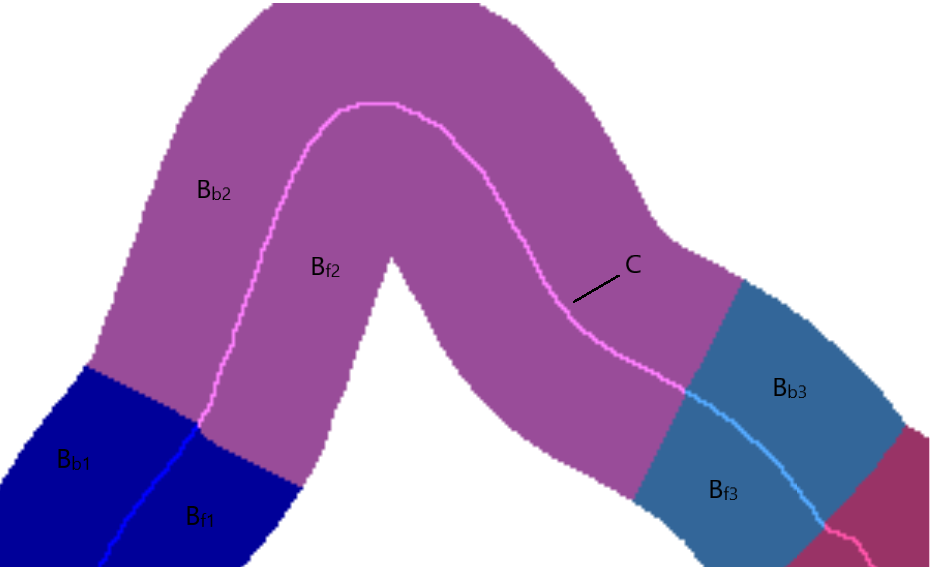
\includegraphics[width=\textwidth]{fig/fb_contour.png}
    \caption{
        Разбиение полосы вокруг контура $\CtLocal$, по которой вычисляется
        функция ошибки, на области $\CtLocalFgI$ и $\CtLocalBgI$
    }
    \label{fig:fb_contour}
\end{figure}

Таким образом, для разбиения полосы достаточно разбить на области точки контура.
Для этого на участки делится поверхность трёхмерной модели объекта: объект
помещается в центр единичной сферы, а сама сфера разбивается на $32$ равные по
площади части по зенитным и азимутным углам.
Каждую точку объекта можно отнормировать, чтобы она попала на поверхность
сферы, и таким образом поделить на области поверхность объекта
(рис.~\ref{fig:color-object-areas}).
Проекция объекта позволяет поделить на области контур
(рис.~\ref{fig:projected-areas}).

\begin{figure}[t]
    \centering
    \begin{minipage}[h]{0.49\linewidth}
        \center{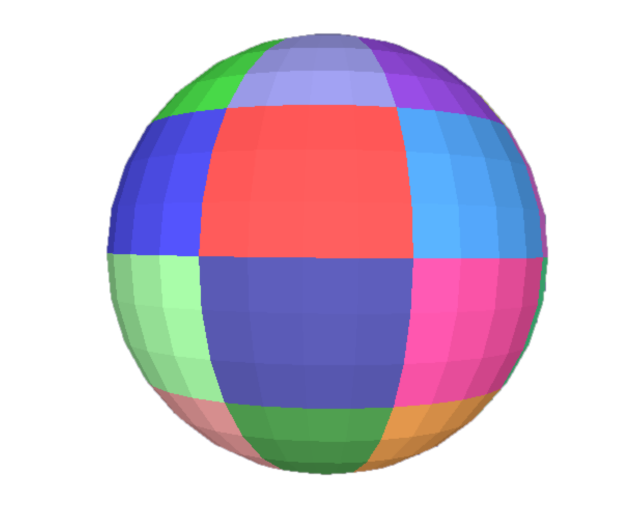
\includegraphics[width=0.8\linewidth]{fig/sphere_straight.png}}
    \end{minipage}
    \hfill
    \begin{minipage}[h]{0.49\linewidth}
        \center{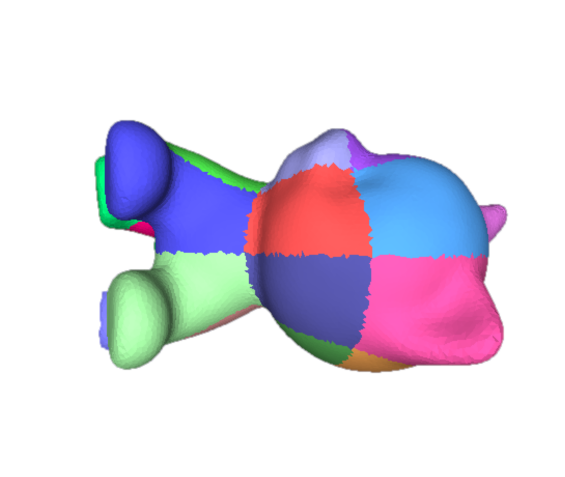
\includegraphics[width=0.8\linewidth]{fig/cat_straight.png}}
    \end{minipage}
    \caption{Разбиение на локальные области поверхностей сферы и объекта}
    \label{fig:color-object-areas}
\end{figure}

\begin{figure}[t]
    \centering
    \begin{minipage}[h]{0.49\linewidth}
        \center{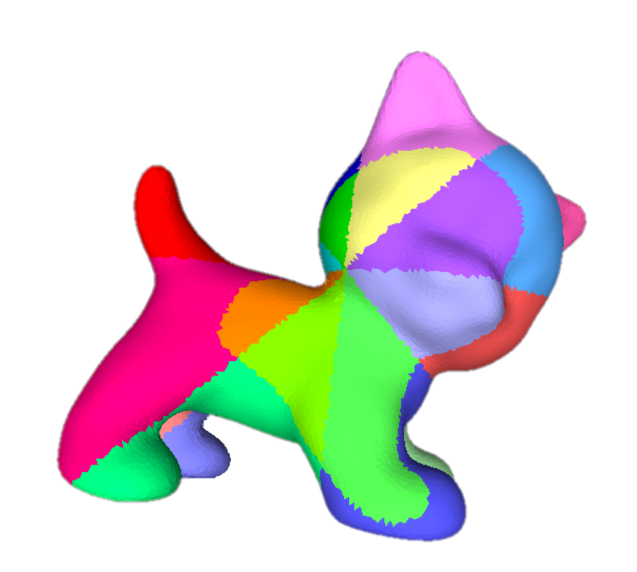
\includegraphics[width=0.8\linewidth]{fig/cat_transformed.png}}
    \end{minipage}
    \hfill
    \begin{minipage}[h]{0.49\linewidth}
        \center{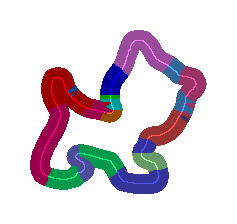
\includegraphics[width=0.8\linewidth]{fig/cat_contour.png}}
    \end{minipage}
    \caption{Слева разбиение на области 3D-модели объекта. Проекция объекта
        разбивает на области контур (правое изображение). Точки вокруг контура
        поппадают в ту же область, что и ближайшие точки на контуре.
    }
    \label{fig:projected-areas}
\end{figure}

Такое разделение объекта неизменно между кадрами, поэтому цветовую информацию
в гистограммах можно накапливать в ходе трекинга.
Данные в гистограммах $\HistLocalFg$ будут при этом отражать распределение
цветов на определённых областях объекта, а данные в гистограммах
$\HistLocalBg$ "--- распределение цветов на фоне вокруг этих областей.
Количество гистограмм не зависит от размера 3D-модели и остаётся небольшим, что
положительно влияет на время работы метода и позволяет обновлять все
гистограммы на каждом кадре.

На локальные области разделяется весь объект целиком.
При этом очевидно, что на отдельном кадре только часть областей будут
спроецированы на контур и поучаствуют в разбиении изображения.
Поэтому информация в некоторых гистограммах может не набираться на протяжении
большого количества кадров.
После поворота объекта такие области могут понадобиться, но информации в
их гистограммах будет недостаточно.

Для решения этой проблемы ведётся учёт \term{опыта} локальных гистограмм и
заводится одна глобальная гистограмма.
Опыт $\ExpLocalI$ локальной пары гистограмм
$\left( \HistLocalFg, \HistLocalBg \right)$
оценивается как общее количество пикселей, попавших
когда-либо в соответсвующую ей область $\CtLocalI$.
Чтобы полученный на старых кадрах опыт учитывался с меньшим весом, чем на
новых, на каждом кадре он домножается на меньший единицы коэффициент:
\begin{equation}
    \ExpLocalI = \CoefFg \ExpLocalINew + (1 - \CoefFg) \ExpLocalIOld
\text{.}
\end{equation}

Если опыт $\ExpLocalI$ меньше некоторого порога $\ExpSuff$,
то вместо значений в локальных гистограммах
$\HistLocalFg$ и $\HistLocalBg$
используются их взвешенные суммы с ячейками глобальных гистограмм
$\HistGlobalFg$ и $\HistGlobalBg$:
\begin{align}\label{eqn:histo_skill}
\Hf(y) &= \dfrac{\ExpLocalI \HistLocalFg + (\ExpSuff - \ExpLocalI)
\HistGlobalFg}{\ExpSuff} \\
\Hb(y) &= \dfrac{\ExpLocalI \HistLocalBg + (\ExpSuff - \ExpLocalI)
\HistGlobalBg}{\ExpSuff}
\text{.}
\end{align}
Порог $\ExpSuff$ выбирается как среднее значение опыта по всем локальным
гистограммам.

\subsection{Комбинирование методов}\label{combining}

\Comment{В чем суть комбинирования, просто поиск исходной позиции ключевыми
точками? Не только: еще и правильное согласование новой позиции и ключевых
точек. Оно заключает в себе: (1) репроецирование новых точек уже из новой
позиции, пересчет старых точек и отбрасывание точек с невидимых граней можно
тоже сюда же записать.}

Предлагаемый подход комбинирования алгоритмов заключается в их последовательном
применении и инициализации одного метода другим.

Ошибки цветового алгоритма часто бывают вызваны тем, что оптимизация функции
энергии сходится к локальному оптимуму.
Этого можно избежать, если точка инициализации достаточно близка к искомому
глобальному минимуму.
Кроме того, хорошая инициализация позволяет сократить время оптимизации
цветовой функции ошибки и повысить общую производительность метода.
Роль такой инициализации в предлагаемом методе играет результат алгоритма
ключевых точек.

С другой стороны, качество работы алгоритма на основе точечных особенностей
сильно зависит от точности вычисления 3D-прообразов ключевых точек.
Она, в свою очередь, зависит от точности позиции объекта в кадрах, на которых
происходит это вычисление, что ведет к опасности накопления ошибки.
Поэтому предлагается использовать оптимизированные цветовым алгоритмом позиции
объекта для вычисления 3D-прообразов новых ключевых точек и уточнения
прообразов старых.

\newcommand{\XOld}{\ensuremath{\xvec_{\text {\it old}}}}
\newcommand{\XNew}{\ensuremath{\xvec_{\text{\it new}}}}
\newcommand{\ReprErr}[1]{\ensuremath{\vect{e}( #1 )}}

Схема комбинирования алгоритмов показана на рис.~\ref{fig:combining_schema}.

\begin{figure}[t]
    \centering
    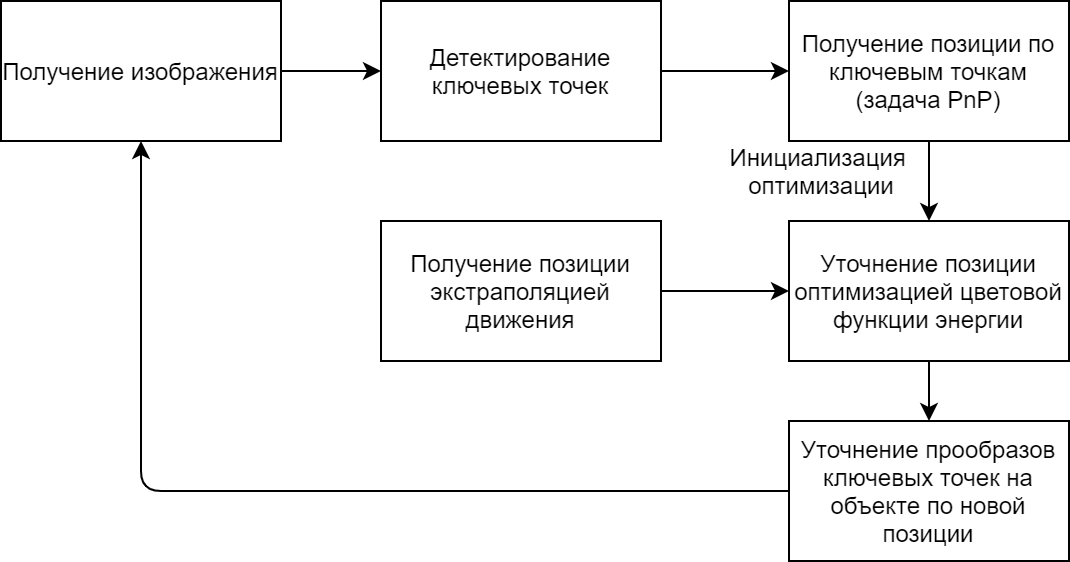
\includegraphics[width=\textwidth]{fig/combining_schema.png}
    \caption{
        Схема комбинирования алгоритмов
    }
    \label{fig:combining_schema}
\end{figure}

На каждом новом кадре позиция объекта сначала вычисляется с помощью
описанного в разделе~\ref{subs:feat_tracking} метода ключевых точек.
При благоприятных условиях данная позиция будет близка к глобальному минимуму
цветовой энергии.
В таком случае выгодно использовать эту позицию как начальную в оптимизации.
Если же метод ключевых точек отработал плохо (например, из-за смазанности
изображения), то такая позиция может оказаться далеко от искомого оптимума и
из нее цветовой алгоритм может не сойтись.
В подобных ситуациях может помочь альтернативный способ вычисления начального
положения, экстраполирующий движение по положениям объекта на двух предыдущих
кадрах.
Из двух возможных начальных позиций для инициализации предлагается выбирать ту,
в которой цветовая функция ошибки покажет меньшее значение.

Оптимизированная цветовым алгоритмом позиция используется в работе с точечными
особенностями.
3D-прообразы обнаруженных впервые ключевых точек строятся уже из этой позиции.
С её помощью также проводится фильтрация выбросов: исключаются из рассмотрения
те 2D-3D-соответствия, для
которых ошибка репроекции из уточнённой позиции больше определённого порога.
Помимо этого, удаляются точки, которые не попадают на передний план, то есть не
лежат на проекции объекта.
Кроме того, при вычислении 3D-прообраза ключевой точки точки запоминается
полигон 3D-модели, на котором он лежит.
Если некоторый полигон не виден на переднем плане, то лежащие на нём точки
считаются невидимыми и тоже далее не рассматриваются.
Таким образом фильтруются 2D-3D соответствия, не согласующиеся с уточненной
цветовым алгоритмом позицией объекта.

Для точек, которые не были отфильтрованы и наблюдались на предыдущих кадрах,
3D-координаты еще раз считаются с
использованием оптимизированной позиции объекта.
Эти новые 3D-координаты ключевой точки заменят старые на следующем кадре, если
будут иметь меньшую ошибку репроекции на изображение.
Пусть $\uvec_{i + 1}$ "--- 2D-координаты точечной особенности на кадре
$\Img_{i + 1}$, а $\xvec$ "--- ее 3D-координаты.
Тогда ошибка репроекции считается как
\begin{equation}\label{eqn:err_reproj}
    \ReprErr{\xvec} = \| \uvec_{i + 1} - \projAt{\Pose_{i + 1}}(\xvec) \|
\end{equation}
Старые 3D-координаты $\XOld$ заменяются на новые $\XNew$, если
$\ReprErr{\XNew} < \ReprErr{\XOld}$.
Сравнивать их сразу же на кадре~$i$ было бы некорректно, так как ошибка
репроекции $\XNew$ на нем нулевая.

Описанные выше действия позволяют согласовать 2D-3D соответствия с уточнённой
позицией.

\Comment{Перенёс описание фильтрации перед пересчётом 3D-позиций. Явно указал,
что пересчёт проводится для неотфильтрованных точек}
